\chapter{Architektur}

\section{Ziele}

Die folgende Architektur soll es ermöglichen, eine Flotte von Drohnen automatisiert und zentralisiert zu verwalten. Die Kommunikation zwischen Server und Drohne muss ausserdem von beiden Seiten initiierbar sein. Zusätzlich muss eine Schnittstelle für Kunden existieren, damit Bestellungen getätigt werden können. 

\section{Übersicht}

Die Abbildung \ref{fig:architecture-overview} zeigt eine Übersicht der verschiedenen Tiers und Server-Komponenten.

\begin{figure}[h]
	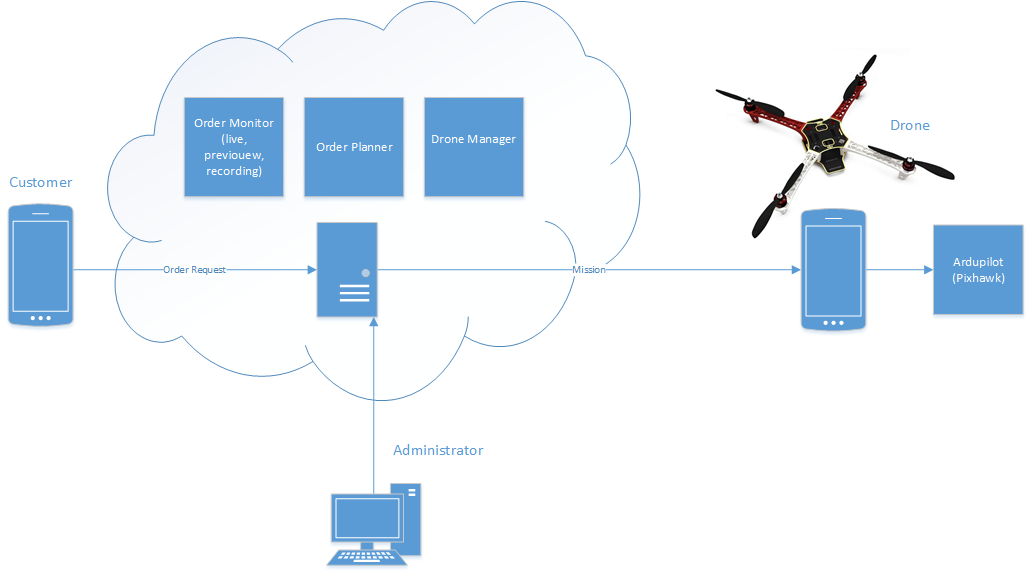
\includegraphics[width=1.0\textwidth]{images/Overview-Diagram.png}
	\caption{Übersicht der Project Helin Architektur }
	\label{fig:architecture-overview}
\end{figure}

\section{Logische Architektur}

\section{Komponenten Übersicht}

Abbildung \ref{fig:logical-architecture-overview} zeigt die Hauptkomponenten, sowie eine Übersicht der enthaltenen Layer und Packages. Ausserdem sind die Abhängigkeiten zu den wichtigsten externen Komponenten dargestellt. Hervorzuheben ist ebenfalls die gemeinsame Verwendung der Messages-Komponente. 

\begin{figure}[h]
	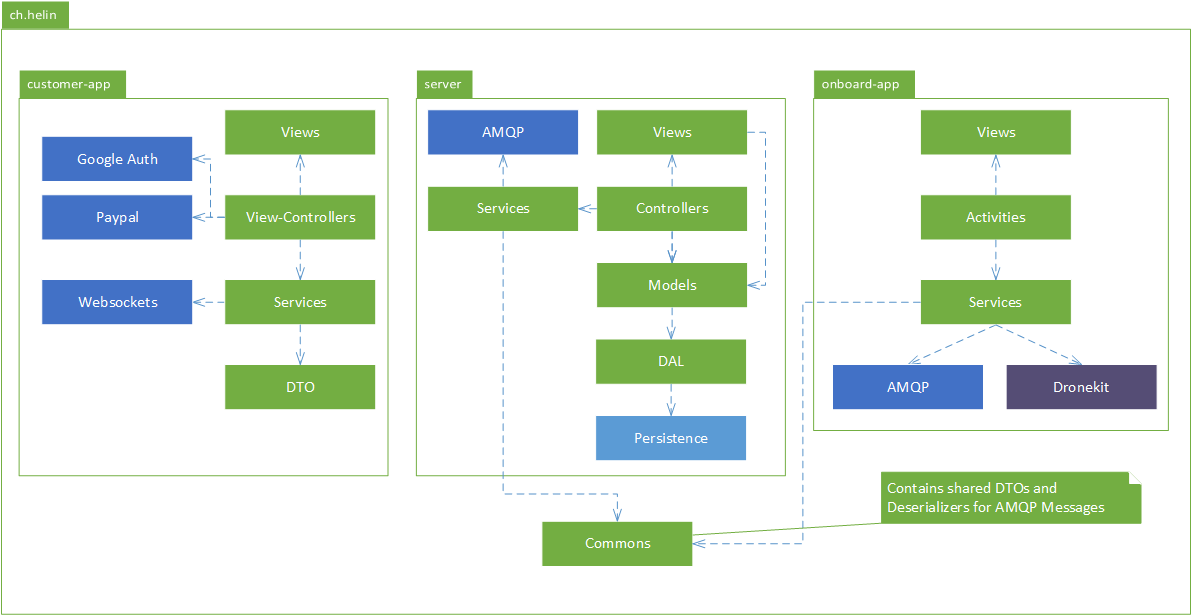
\includegraphics[width=1.0\textwidth]{images/logical-architecture-overview.png}
	\caption{Vereinfachte Übersicht der logischen Architektur und deren Komponenten }
	\label{fig:logical-architecture-overview}
\end{figure}

\section{Server-Komponente}

\subsection{Anforderungen}
%Todo sauber referenzieren
Aus den in den Anforderungen definierten Zielen, ergeben sich für die Server-Komponente folgende Anforderungen:

\begin{itemize}
	\item Bietet Benutzeroberfläche für Administratoren
	\item Verwaltet CRUD für alle nötigen Klassen (siehe Domain Model)
	\item Verwaltet Verbindungen zu Onboard-Apps und Customer-Apps
	\item Berechnet Flugrouten basierend auf den erhaltenen Bestellungs-Koordinaten
\end{itemize}

\subsection{Layers}
Die Architektur des Servers basiert auf dem {MVC Pattern \cite{MVC}}, da dieses für CRUD Applikationen mit Benutzeroberfläche besonders geeignet ist und dafür viele geeignete Frameworks zur Verfügung stehen.\\

Für Komponenten die aus unterschiedlichen Controllern verwendet werden, wurde zusätzlich eine Service Komponente verwendet. Die Services stellen Abstraktionen für wichtige Funktionen wie das Messaging und die Routenberechnung bereit.

Die Verantwortlichkeiten und Kollaborationen der Layer werden nachfolgend genauer definiert.

\subsubsection{View-Layer}
Stellt die grafische Benutzeroberfläche zur Verfügung und rendert diese basierend auf den Model-Daten.

\subsubsection{Controller-Layer}
\begin{tabular}{|p{.70\textwidth}|p{.30\textwidth}|} \hline
	\textbf{Verantwortlichkeiten} & \textbf{Zusammenarbeit} \\ \hline \hline
	\begin{itemize}
		\item Lädt Daten für Views aus dem Data-Access-Layer
		\item Verarbeitet eingehende HTTP-Requests
		\item Verarbeitet eingehende Messages aus den Messaging-Queues
		\item Enthält Business-Logik und steuert Ablauf nach einem Request	
	\end{itemize}&
	\begin{itemize}
		\item Data-Access-Layer
		\item Service-Layer
		\item Model-Layer
		\item Messages
	\end{itemize}
	\\ \hline
\end{tabular}

\subsubsection{Model-Layer}

Der Model-Layer enthält die Datenmodelle. (siehe Domain Model)

\subsubsection{Service-Komponente}

\begin{tabular}{|p{.70\textwidth}|p{.30\textwidth}|} \hline
	\textbf{Verantwortlichkeiten} & \textbf{Zusammenarbeit} \\ \hline \hline
	
	\begin{itemize}
		\item Verwaltet Verbindungen zu den Drohnen
		\item Deserialisiert eingehende Nachrichten
		\item Leitet eingehende Nachrichten von Drohnen an den Controller-Layer weiter	
		\item Leitet eingehende Nachrichten von Customers an den Controller-Layer weiter	
		\item Berechnet Flugrouten basierend auf den vorgegebenen Flugzonen
	\end{itemize}&
	\begin{itemize}
		\item Controller-Layer
		\item AMQP-Library
		\item Messages
	\end{itemize}
	\\ \hline
\end{tabular}

\subsubsection{Data-Access-Layer (DAL)}

Der Data Access Layer bietet die Möglichkeit auf die Persistence Library zuzugreifen und stellt dafür die wichtigsten Funktionen zur Verfügung. 

\section{Onboard-App}

\subsection{Anforderungen}

\begin{itemize}
	\item Kommuniziert mit dem Flight-Controller der Drohne
	\item Kommuniziert mit dem Server
	\item Bietet eine Benutzeroberfläche für den Drone-Operator 
\end{itemize}

\subsection{Layer}

Die App enthält die normalen Android-Application-Layer wie Activities und Views. Zusätzlich kommt der Service-Layer hinzu. Dieser enthält keine Android-Services, sondern selbst entwickelte Service-Klassen.

\subsubsection{Service-Komponente}

\begin{tabular}{|p{.70\textwidth}|p{.30\textwidth}|} \hline
	\textbf{Verantwortlichkeiten} & \textbf{Zusammenarbeit} \\ \hline \hline
	
	\begin{itemize}
		\item Verwaltet Verbindung zur Drohne
		\item Verwaltet Verbindung zum Server
		\item Deserialisiert eingehende Nachrichten.
		\item Leitet eingehende Nachrichten vom Server and den Activities-Layer oder andere Services weiter
		\item Ermöglicht das Senden von Nachrichten an den Server
	\end{itemize}&
	\begin{itemize}
		\item Activities-Layer
		\item AMQP-Library
		\item Messages
	\end{itemize}
	\\ \hline
\end{tabular}


\section{Customer-App}

\subsection{Anforderungen}

\begin{itemize}
	\item Kommuniziert mit dem Server
	\item Bietet eine Benutzeroberfläche für den Customer
\end{itemize}

\subsection{Layer}

Die App enthält die normalen Android-Application-Layer wie Activities und Views. Zusätzlich kommt der Service-Layer hinzu. Dieser enthält keine Android-Services, sondern selbst entwickelte Service-Klassen.

\subsubsection{Service-Layer}

% TODO AMQP is wrong betwen server and customer app
\begin{tabular}{|p{.70\textwidth}|p{.30\textwidth}|} \hline
	\textbf{Verantwortlichkeiten} & \textbf{Zusammenarbeit} \\ \hline \hline
	
	\begin{itemize}
		\item Verwaltet Verbindung zum Server
		\item Deserialisiert eingehende Nachrichten.
		\item Leitet eingehende Nachrichten vom Server and den Activities-Layer weiter
		\item Ermöglicht das Senden von Nachrichten an den Server
	\end{itemize}&
	\begin{itemize}
		\item Activities-Layer
		\item AMQP-Library
		\item Messages
	\end{itemize}
	\\ \hline
\end{tabular}

\subsubsection{HTTP statt RabbitMQ}
Bei der Kommunikation vom Onboard-App zum Server wurde auf AMQP gesetzt, da sowohl die Drohne als auch der Server die Möglichkeit haben sollten bidirektional Daten auszutauschen. 
Für den Customer-App war auch AMQP eingeplant. Aufgrund vom Einsatz von Xamarin und C-Sharp wurde dies neu evaluiert, wie der Support für RabbitMQ ist.
Es existiert ein Library für C-Shapr \cite{easynetq}, jedoch ist die Verwendung innerhalb von Xamarin.Forms nicht verbreitet \cite{ampq-csharp}. 

Aufgrund dessen wurde auf HTTP und Websocket gesetzt.
Denn für den Customer-App überwiegen die Vorteile von AMQP nicht deren von HTTP:
\begin{itemize}
	\item{
		Beim Verbindungsabbruch ist der Verlust einer Nachricht nicht schlimm.
		Dem Benutzer kann einer Nachricht gezeigt werden und dieser kann auf Wunsch die Anfrage nochmals verschicken}
	\item{
		Alle Anfragen werden nur von App an den Server verschickt.
		Einzig die aktuelle Position der Drohne sollte vom Server an den Kunden geschickt werden können.
		Dies kann auch mittels Pulling gelöst werden, denn für den Kunden ist dies nicht spürbar.
		Es können alle paar Sekunden eine Anfrage an den Server geschickt zu werden.
		Serverseit ist die Mehrlast auch zu vernachlässigen, da die Anfrange nur geschickt werden,
		falls eine aktuelle Mission läuft.
	}
\end{itemize}

HTTP gegenüber AMQP hat noch den Vorteil, dass die REST Schnittstelle, einfacher von einem drittanbieter verwendet werden können.

\section{Kommunikations-Architektur}
Die Abbildung \ref{fig:communication-architecture-overview} zeigt die Kommunikations-Architektur in der Übersicht. Wichtig sind vor allem die verschiedenen verwendeten Protokolle, die benötigt werden um die Anforderungen erfüllen zu können. Bei den mobilen Geräten wird Messaging ({\Gls{AMQP}) verwendet, um bidirektionale Kommunikation zu ermöglichen. Dies ist nötig, damit Kunden und Administratoren die Bewegungen der Drohne live verfolgen können. Die eingesetzte Technologie für die Kommunikation zwischen dem Server und den Smartphones muss ausserdem den Nicht-Funktionalen-Anforderungen gerecht werden im Bezug auf Verbindungsabbrüche und Verbindungswiederherstellung.

\begin{figure}[H]
	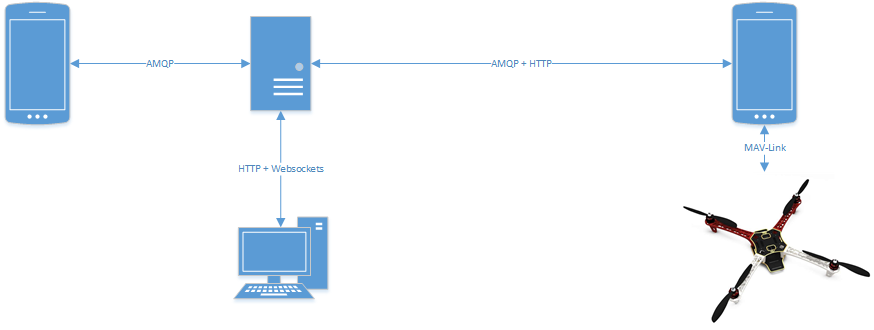
\includegraphics[width=1.0\textwidth]{images/Communication-Overview-Diagram.png}
	\caption{Übersicht der Kommunikations-Architektur mit den jeweiligen Protokollen. }
	\label{fig:communication-architecture-overview}
\end{figure}

\subsection{Verwendete Enterprise Integration Patterns}
Messaging-Systeme und Protokolle bieten eine grosse Auswahl an Patterns die je nach Anforderungen verwendet werden können.({\cite{EIP}}) Für dieses Projekt benötigen wir nur einen kleinen Teil davon um den gestellten Anforderungen gerecht zu werden.
%
\subsubsection{Point-to-Point Channel}
Um zwischen einer registrierten Drohne und dem Server einen sicheren und zuverlässigen Nachrichtenaustausch zu ermöglichen, wird jede Drohne bzw. jede App über einen separaten Point-to-Point Channel	\cite[S. 103]{EIP}} angebunden. Der Channel wird nach der Registrierung zugeteilt und stellt den Point-to-Point Kanal zwischen Drone und Server dar. Dies garantiert dem Server eine Nachricht an garantiert eine Drohne zu schicken.
%
\subsubsection{At-most-once}

Die Fehlersemantik At-most-once gibt die Sicherheit dass eine Drohne eine Mission oder einen Befehl nur ein Mal erhält. Ansonsten müsste das System idempotent gebaut werden. Exactly-once delivery ist in der Praxis eigentlich unmöglich umzusetzen, weshalb wir uns für diese Alternative entschieden haben. 
%
\subsubsection{Event-driven Consumer}
{Event-driven Consumer \cite[S. 442]{EIP}} Systeme bieten die Möglichkeit auf Grund von Nachrichten Aktionen auszuführen. Beispielsweise:
%
\begin{itemize}
	\item Drohne erhält neue Mission vom Server und soll dies dem Drone-Operator anzeigen.
	\item Server erhält neue Position von der Drohne und soll diese Nachricht dem Kunden weiterleiten und dem Administrator auf dem Web-Client anzeigen.
	\item Smartphone des Kunden erhält neue Position der Drohne, auf der Karte wird die Position der Drohne angezeigt.
\end{itemize}


\subsection{Register Drone}
%TODO gehört in die Umsetzung
\begin{figure}[h]
	\centering
	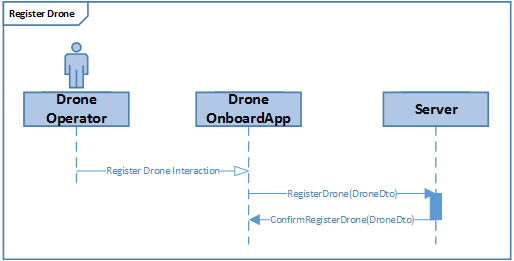
\includegraphics[scale=1.0]{images/registerDrone.png}
	\caption{Übersicht der Project Helin Architektur }
	\label{fig:registerDrone}
\end{figure}
%
\subsection{Order Cargo}
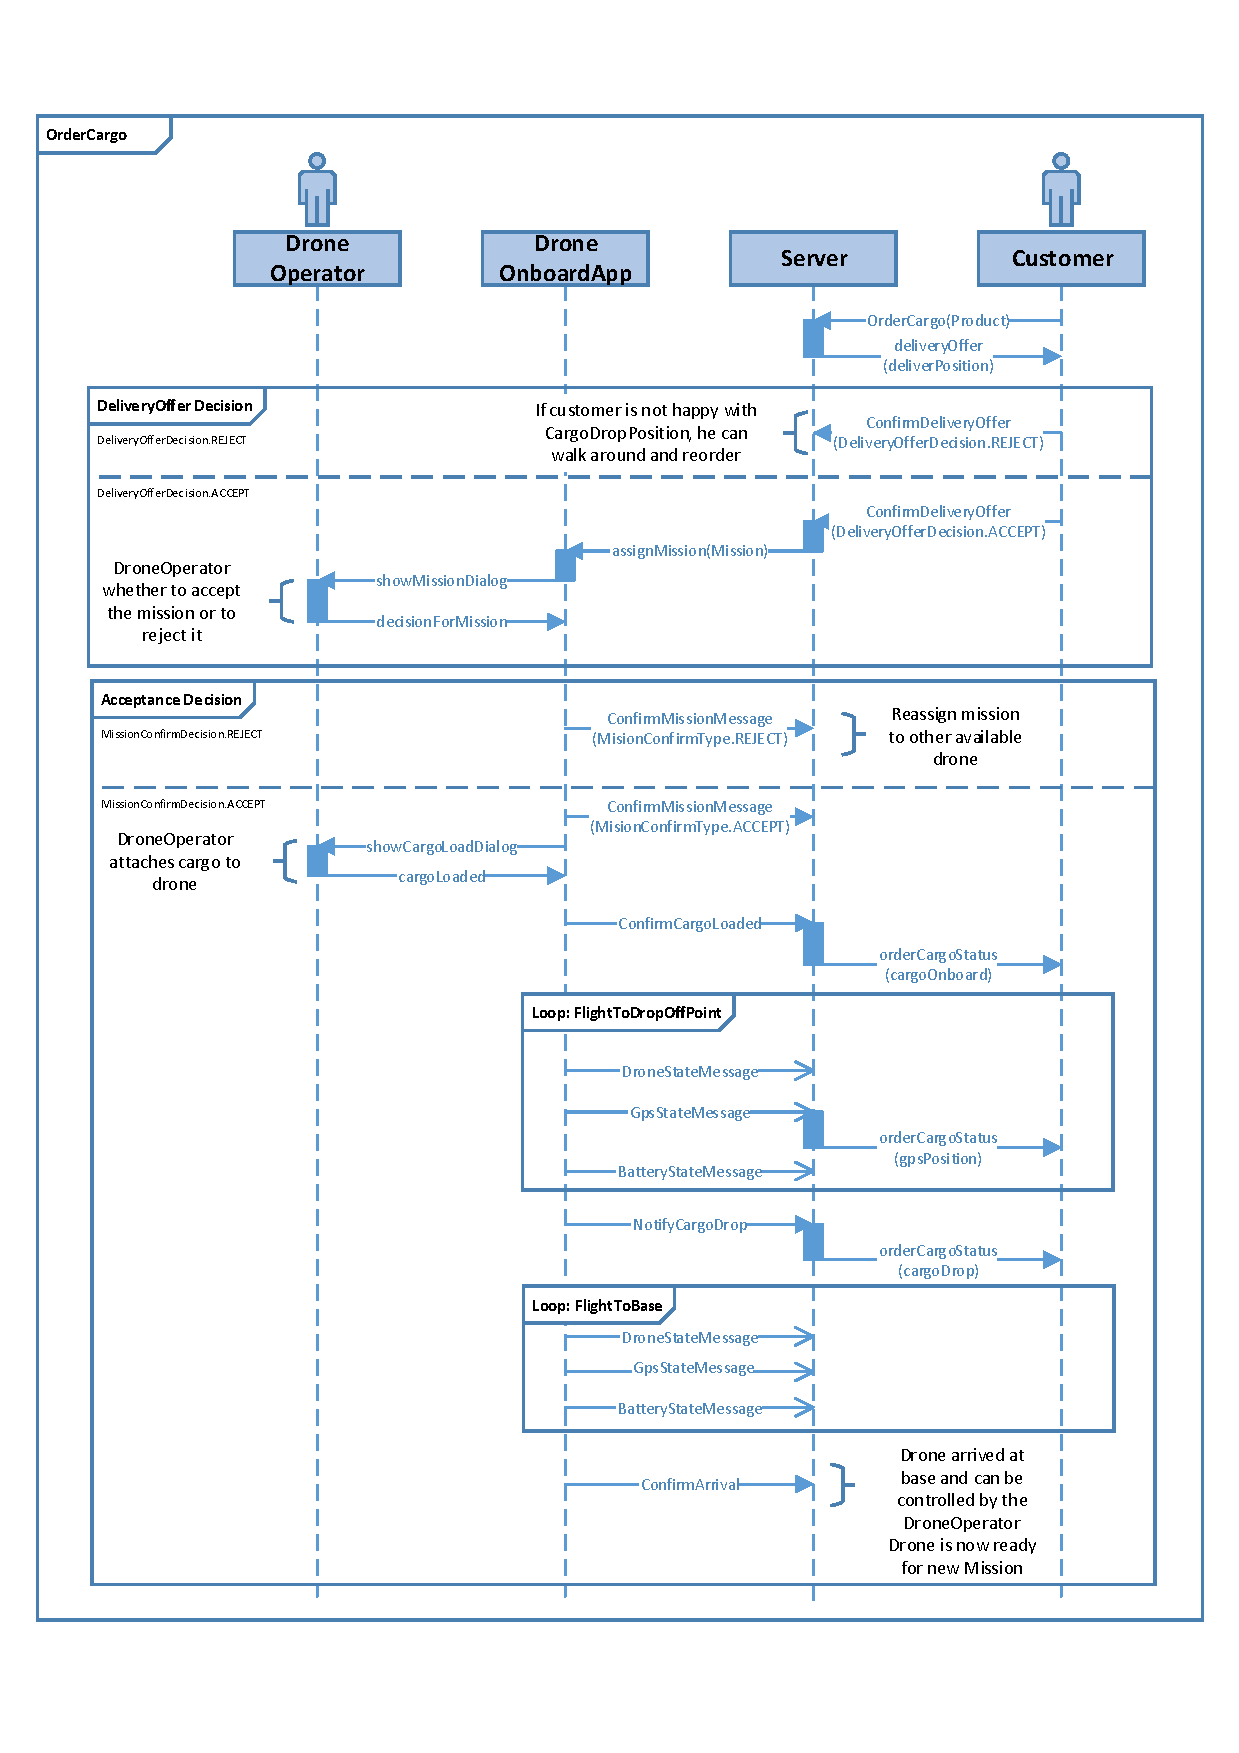
\includepdf[pages=-]{images/OrderCargo.pdf}
Order Cargo (Abbildung \ref{fig:registerDrone}) beschreibt den Bestellprozess und die damit zusammenhängende Kommunikation. \\
Der User möchte gerne an einem Anlass ein Produkt bestellen. Er bestellt mittels der App ein Produkt, der Server bestätigt ihm die Bestellung und schlägt einen Abwurfort vor. Sollte der Abwurfort dem Kunden nicht entsprechen, so kann er den Prozess abbrechen und ihn nocheinmal auslösen, sobald er sich in einer geografisch glücklicheren Lage befindet.
\\
Der Server evaluiert im Anschluss eine verfügbare Drone, welche den Auftrag ausführen kann und schlägt die Mission dem DroneOperator vor. Sollte die Drone verfügbar sein, so kann er diesen Auftrag bestätigen. Im Fall einer Wartungsarbeit kann der Auftrag zu diesem Zeitpunkt auch abgelehnt werden. Sobald der Auftrag angeommen wurde, erhält der DroneOperator genaue Angaben zur Beladung der Drohne. Anschliessend wird die Ladung bestätigt und der Server kann dem Kunden mitteilen, dass die Drone nun startklar ist. Während des Fluges erhält der Kunde Benachrichtigungen vom Server mit der aktuellen Position der Drohne. Sobald die Ladung abwurfbereit ist, wird der Kunde informiert und die Drohne kann die Ladung abwerfen. Im Anschluss fliegt die Drohen zur Basis zurück und bestätigt dem Server die Ankunft. So kann gewährleistet werden, dass die Drohne wieder eine eine Mission erhalten kann.
%